Compilers usually have one or more data structures known as
\emph{symbol tables}, which are mappings from symbols to information
about the symbol.  In contrast, GHC avoids symbol tables:  instead, a
symbol \emph{contains} all information about itself, forming an
immutable \emph{cyclic data structure} of all symbols
known to GHC\@.  This graph is very convenient to work
with in a purely functional language like Haskell, since queries can
be answered by a direct field access rather than a lookup in
a symbol table.  GHC uses a technique called ``tying the knot''
to construct this graph.

The problem with these types of cyclic data structures is that
they are very difficult to update.  Fortunately, GHC rarely
needs to update information in the graph; the graph just grows
monotonically in size as we typecheck declarations.
Unfortunately, sometimes an update is necessary---for example, when
we compile the \verb|hs| file for an \verb|hs-boot| file, we
need to update our graph with the new information about all the
symbols.  GHC's handles such situations by throwing out the out-of-date
portion of the graph and rebuilding it from scratch.

Tying the knot for this cyclic data structure is a dark corner of GHC\@.
It is a relatively straightforward to tie the knot when loading
interface files from disk---but there is also the subtle case when we
compile an \verb|hs| file which has an associated \verb|hs-boot| file:
in this case, the knot is tied \emph{across} type checking itself.
The purpose of this paper is to shed some light on how this all works.
Specifically:

\begin{itemize}
    \item We describe GHC's \emph{graph representation} (Section~\ref{sec:graph}), in
    which there are no symbol tables, contrast it with
    the \emph{interface representation} (Section~\ref{sec:interface}), which utilizes symbol
    tables, is serialized to disk, and describe how we convert
    between these two representations (Section~\ref{sec:convert}).  Most operations like type
    equality are implemented only for the graph representation, but
    operations which involve \emph{updating} information associated with
    a symbol can only conveniently be done on the interface
    representation.

    \item We describe the process for typechecking
    \verb|hs-boot| files (Section~\ref{sec:boot}). The
    difficulty is that the incomplete symbols supplied
    by the \verb|hs-boot| file must eventually be improved
    with the information from their implementations in the
    \verb|hs| file.  In this case, GHC ties the knot \emph{across}
    typechecking itself.  Although GHC does not support
    using type synonyms to implement abstract data types, it turns out that
    this knot tying accidentally solves the double vision
    problem in the same way as Dreyer's recursive module
    calculus (RMC).

    \item What invariants do we expect this graph to uphold?
    If the user's source code is well-typed, we definitely expect
    the graph to generally make sense (e.g., be well-typed and
    well-kinded).  But what if the user's code is ill-typed?  We
    might still hope that GHC can enforce consistency by refusing
    to add malformed types to the graph.  Unfortunately, with
    knot-tying for \verb|hs-boot| files, it is easy to construct
    malformed types.  Fortunately, such malformed types can occur in RMC
    as well and do not seem to cause soundness problems.  However, GHC
    does have to be careful to avoid type synonym cycles, which can
    cause the compiler to loop.

    \item The typechecking algorithm for Backpack requires
    a number of operations on GHC's representation of types:
    \emph{substitution}, \emph{type matching} and \emph{merging}.
    We carefully spell out what these operations are, and give
    the strategy for implementing these operations in GHC\@.
\end{itemize}

\section{Graph representation (without symbol tables)}
\label{sec:graph}

The \emph{graph representation} for types embeds information about
symbols inside the data structure itself.  For example, here are
some data types for the graph representation from GHC (simplified
and abbreviated):

\begin{verbatim}
    data Type  = TyConApp TyCon [Type]  | ...
    data TyCon = SynonymTyCon Name Type | ...
    data ModDetails = ModDetails [TyCon] ...
\end{verbatim}

\noindent
A type may be an application of a type constructor to some arguments, in which
case it contains a type constructor \verb|TyCon|.  A type constructor
can be a type synonym, in which case it contains the type it expands
to.  A module \verb|ModDetails| consists of a list of type constructors
and other entities that are defined in it.  The ``graph'' is the graph of
heap objects which represent these data types.

It is very convenient to write algorithms which operate on the graph
representation, as any query which would have required a lookup in
a symbol table are reduced to a simple field access, improving efficiency
and code clarity.  For example, type equality can be defined as a
pure function \verb|Type -> Type -> Bool| even in the presence of type
synonyms, since the \verb|SynonymTyCon| always carries along the expanded
version of the synonym to compare against.

\section{Interface representation (with symbol tables)}
\label{sec:interface}

The \emph{interface representation} for types does not
embed information in its types, and thus is suitable
for serialization to binary interface files.  For example,
here are some data types for the interface representation
(also simplified):

\begin{verbatim}
    data IfaceType = IfaceTyConApp Name [IfaceType] | ...
    data IfaceDecl = IfaceSynonym OccName IfaceType | ...
    data ModIface = ModIface [IfaceDecl] ...
\end{verbatim}

\noindent
Unlike the graph representation, the type constructor application
doesn't embed the definition of the type constructor---instead,
it records only a \verb|Name| reference to the constructor. To find out
more information about the type constructor, you would have to lookup
the \verb|IfaceDecl| from the appropriate symbol table; e.g., a module
local declaration would be found in the \verb|IfaceDecl| list in
\verb|ModIface|.

It is much harder to directly test for type equality on interface types.
We can't write a pure function \verb|IfaceType -> IfaceType -> Bool|
---in the presence of type synonyms, we may need to do a lookup in
a symbol table to determine how the synonym expands.  However, it is
very easy to update an \verb|IfaceDecl|, since the information
associated with it is centralized in one place.

\section{Converting between representations}
\label{sec:convert}

\paragraph{Conversion from graph to interface}  We convert from
the graph representation to the interface representation when we
are ready to serialize the results of typechecking to disk.
This process is fairly straightforward: all structures in the graph
representation record a globally unique name identifying them,
so we simply drop the extra information and preserve only the name.

\paragraph{Conversion from interface to graph} How do we convert from
the interface representation to the graph representation?  An important
point is that this conversion process doesn't happen in isolation. You
can't just simply convert an
\verb|IfaceType| into a \verb|Type|: where should a
\verb|Name| reference be resolved to?  You need a
symbol table---one which records the graph nodes of any \verb|Name| you
may refer to.  Thus, this conversion is always done with respect to
some graph; GHC largely assumes that there is only one such graph,
and that it is populated with all dependencies. GHC gives this
illusion by lazily \emph{loading} declarations into the graph
when needed; indeed, this is the usual reason an interface is
being converted into graph representation.

In the GHC codebase, the process of converting from interfaces to
the graph representation is called \emph{type checking} (though this
is not a very good name, since this process never fails---the
interface file is assumed to be well-typed).

\section{Tying the knot for hs-boot files}
\label{sec:boot}

\verb|hs-boot| files pose a special problem for the graph
representation, because they require an \emph{update} to the
graph representation.  For example, suppose we are typechecking
the source files \verb|A.hs-boot|, \verb|B.hs| and \verb|A.hs|:

\begin{enumerate}
    \item We typecheck \verb|A.hs-boot|, producing an \emph{incomplete}
    graph for the types and values defined in this
    file.  This graph is incomplete because its type
    constructors may lack information about data type constructors (the
    user defined an abstract data type); similarly, its values may lack
    unfoldings (there is no source code in an \verb|hs-boot| file).

    \item We typecheck \verb|B.hs|.  The graph we build for this module
    refers to the incomplete graph from \verb|A.hs-boot|.

    \item We typecheck \verb|A.hs|, producing the complete graph
    for these types and values, while simultaneously
    updating the references on all the modules from step (2) to point
    to the new, complete graph. This update is called
    \emph{re-typechecking}, for reasons that will become clear soon.
\end{enumerate}

\noindent
The evolution of the graph representation is shown diagramatically below.
In the first column, we have the source code being compiled (bottom-first).
We typecheck \verb|A.hs-boot| and \verb|B.hs|, forming an incomplete graph
(second column), as well as some interface files (third column).
When we finally typecheck \verb|A.hs|, we simultaneously retypecheck
the interface file \verb|B.hi|, allowing us to tie the knot between the
graph representations for \verb|T| and \verb|S|, discarding the old
graph (which is now out of date.)

\begin{figure}[H]
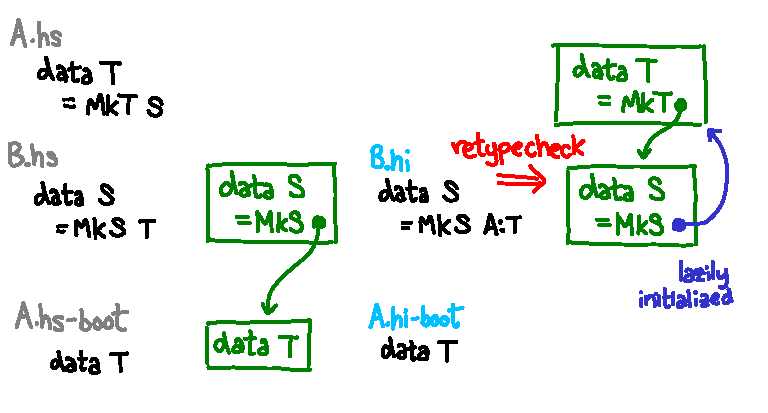
\includegraphics{hs-boot-diagram.pdf}
\end{figure}

\noindent
Tying the knot is easy to do if we have an up-to-date copy of \verb|A.hi| in
hand (not shown), but what if we are typechecking \verb|A.hs| to generate the
interface file in the first place?  Here lies a dark and twisty corner
of GHC's implementation: we need the updated graph for \verb|data S| in order to typecheck
\verb|A.hs|, but prior to typechecking \verb|A.hs|, we don't actually have
an object representing \verb|data T|.

The solution is to be lazy: we just need to delay committing to the
destination of \verb|data S|'s pointer until we have created the graph node
for \verb|data T|.  Thus, the pointer is initialized with an unsafe thunk
which queries the local type environment for the necessary graph node
when it is forced.  This
is very delicate: if we force the thunk too early, typechecking may not
have built the structure we need and we'll get an error.  This is a big source of bugs!\footnote{\url{https://ghc.haskell.org/trac/ghc/search?q=tcifaceglobal}}  In fact,
\verb|ghc --make| doesn't tie the knot at all; the behavior in these
two cases is inconsistent.

\section{Graph well-formedness and hs-boot}

When studying type-checking algorithms, one is usually concerned with the
properties one gets when the provided programs are \emph{well-typed}.
But of course, real world programs are often ill-typed, and any real
implementation also cares about the behavior of their type-checker on
these programs.  Here is one \emph{property} which we would like our
graph representation to uphold: \emph{all types in the graph
are well-formed}, no matter what inputs the user gives
us.  If a user provides us something bad, we should refuse to
build a graph for it.

Unfortunately, this property is not upheld by the current \verb|hs-boot|
implementation.  Consider this example:

\begin{verbatim}
    -- A.hs-boot
    module A where
        data T
        f :: T -> T
    -- B.hs
    module B where
        import {-# SOURCE #-} A
    -- A.hs
    module A where
        import B
        data T a = T a
        f :: T a -> T a
        f x = x
\end{verbatim}

GHC will stodgily report that the \verb|hs-boot| file's
\verb|f :: T -> T| does not match \verb|f :: T a -> T a|.
Worse yet, due to the knot tying trick, the \verb|T| in
\verb|f :: T -> T| refers to the type constructor for
\verb|data T a = T a|; i.e., the type is ill-kinded!
The problem is that we must commit to knot-tying \verb|T| to
the type presently being typechecked prior to
knowing whether or not the \verb|T|'s kind even matches the
kind in the \verb|hs-boot| file.

Worse yet, you can convince GHC to construct a type synonym
loop and then infinite loop:

\begin{verbatim}
    -- A.hs-boot
    module A where
    data S
    type R = S
    -- B.hs
    module B (module A, module B) where
    import {-# SOURCE #-} A
    type U = S
    -- A.hs
    module A where
    import qualified B
    type S = B.R
    type R = B.U
\end{verbatim}

Here, the type synonym \verb|S| in \verb|A.hs| is eagerly wired up
with the occurrences of \verb|S| in \verb|B.hi|, even though
a type synonym is not a valid replacement for an abstract
data type.

So what should we do?  There seem to be two possibilities:

\paragraph{Accept that sometimes the graph will be malformed}  We could
say that there is no problem with GHC today; sometimes the graph will be
ill-kinded or the compiler will loop but the cure is worse than the
disease.  Before we typechecking finishes, we will discover the problem
and bale out (or infinite loop, as the case may be).

\paragraph{Don't tie the knot until after all typechecking is finished}
Intuitively, the reason why we build the bad graph is because we
eagerly rebuild the graph to point to the graph we are typechecking,
before we even know whether or not it makes sense or not.  So an
alternate solution is to \emph{not} tie the knot until we know
if the modification makes sense.  The very simplest implementation
of this strategy would be to just turn off all knot tying, and
retypecheck only after typechecking is completely finished.

There is a decent amount of evidence that this would be a good
idea:

\begin{itemize}
    \item \verb|ghc --make|, by far the most used mode of GHC,
    doesn't correctly tie the knot, and no one has really complained;
    subsequently, some bugs\footnote{https://ghc.haskell.org/trac/ghc/ticket/12042}%
\footnote{https://ghc.haskell.org/trac/ghc/ticket/10083}
    don't affect \verb|ghc --make| (but do affect \verb|ghc -c|).
    \item When Simon Marlow introduced the knot-tying code for
one-shot mode in commit \verb|d83e1ac43a| to fix a subtle ``bug'',
he observed that this bug didn't actually break real code, it just
caused some fingerprints to wobble.
    \item Tying the knot for \verb|Id|s is not very useful,
    because the optimizer is going to update the unfoldings, etc.
\end{itemize}

\noindent
One downside is that without tying the knot, in a hypothetical
extension of \verb|hs-boot| files to support implement abstract
data types with type synonyms, we encounter the double vision problem:

\begin{verbatim}
    -- A.hs-boot
    module A where
        data A
    -- B.hs
    module B where
        import {-# SOURCE #-} A
        f :: A -> A
        f x = x
    -- A.hs
    module A where
        import B
        type A = Int
        y = f (2 :: Int) -- error!
\end{verbatim}

\noindent
Although we have defined \verb|type A = Int|, \verb|y| will fail to
typecheck because the \verb|TyCon| in \verb|f|'s type is abstract and
doesn't contain the necessary unfolding.

\section{The operations Backpack requires}

Let us now characterize the operations Backpack requires on
GHC's representations of types.  For concreteness, we'll consider
how to typecheck the following \textsf{include} statement from Backpack'14:

\begin{verbatim}
    package p where
        A :: [ data T ]
        B :: [ import A; data S = MkS T ]
    package q where
        A = [ data T = MkT ]
        B :: [ data S; f :: S -> S ]
        include p -- *
\end{verbatim}

\noindent
The procedure is as follows:

\begin{enumerate}
    \item The package we are including is associated with some module types
    which are universally quantified over the identities of its holes.
    We first apply a \textbf{substitution} to these module types, updating these
    identities to the actual names the holes are instantiated with.
    In the above example, we substitute \verb|T| in \verb|p| so
    that it refers to the \verb|T| implemented in \verb|q|.  (In Backpack'14,
    this would be substituting $\beta_{AT} \mapsto \nu_A$; in
    Backpack'16 this would be substituting $\nhv{A.T} \mapsto \MOD{q}{\subst{B}{\hv{B}}}{A}.\mathtt{T}$.)

    \item The resulting module types are \textbf{merged}
    into the existing types in the context.  In the above example, the \verb|data S|
    from \verb|q|'s signature is merged with \verb|data S = MkS T| from
    \verb|p|'s signature.  This merge operation may fail, e.g., if
    the types or kinds of the merged declarations do not match; thus,
    there is implicitly a \textbf{type matching} operation which tests
    if the merge will be successful.  (The reason for this separation
    will become clear shortly.)
\end{enumerate}

\noindent
So, which representations are most suitable for these operations?

\begin{itemize}
    \item \textbf{Substitution} is reasonably simple enough to carry out
        on types in either representation.  However, substituting over
        type constructors is most easily done in the \emph{interface
        representation}, because it represents an update to information
        which may be embedded elsewhere in the graph representation.

    \item \textbf{Type matching} involves type equality tests, thus
        it should be done in the \emph{graph representation}.

    \item \textbf{Merging} can cause the information for
        type constructors to be updated; thus, it should be done in the
        \emph{interface representation}.
\end{itemize}

\noindent
The technical difficulty arises from the fact that, although most operations
are most naturally carried out on the interface representation, to
test for type matching, we need to convert to the graph representation
so that we can test for type equality.

\iffalse{}

\section{Type synonyms for Backpack}

In Backpack'14, it is not possible to implement an abstract
data type \verb|data T| with a type synonym \verb|type T = Bool|.
This is a \emph{big} problem in practice, because many existing
types in the Haskell ecosystem we would like to abstract over
were not named the same way (e.g., \verb|String|, \verb|Text|
and \verb|ByteString|).

In the absence of recursion, type synonyms seem to be implementable
quite straightforwardly.  We add a new form of defined entity
specification, $\verb|type|~T = \I{typ}$.  The $T$ is a defined
entity in its own right and can be referred to via an original
name; it just so happens that Haskell type equality is defined
modulo type synonyms.  Indeed, in my F-ing semantics for Explicit
Backpack, I show that this poses no problem.  Of course, we need to
check that we don't allow cyclic type synonyms, but that is old news.

\section{Whither the proofs}

\begin{quote}
``Even \emph{stating} soundness required us to define a formal semantics
for separate typechecking of (recursive) Haskell modules, which did not
exist previously.'' --- Backpack'14
\end{quote}

\noindent
The soundness of Backpack'14 is established by an elaboration to ``a set
of ordinary modules and module types'' (i.e., binary interface files).
In principle, the elaboration should also be a way to implement
Backpack'14.  Clearly, an implementation will not generally employ the
elaboration directly (e.g., you wouldn't actually rewrite source
code of modules), but if the implementation is not too far from
the elaboration (which is proven correct), we have some evidence
that the implementation is also correct.

A question one might ask, then is what would happen if you implemented
Backpack'14 by way of its elaboration?  This process is quite
involved, because the elaboration must produce not only Haskell source
files (the ``ordinary modules''), but also binary interface files (the
``module types'').  This can be most clearly seen in the following
example:

\begin{verbatim}
    package p where
        A = [x = True]
        B = [import A; y = not x]
\end{verbatim}

\noindent
There is nothing interested going on with this example; na\"\i vely,
we would expect our ``elaboration'' ought to be a no-op.  This
is \emph{not the case}!  When Backpack'14 performs an elaboration,
it elaborates every module declaration to both a Haskell module
\emph{and} a module type.  To put it differently, we need to produce
both a Haskell source file \emph{and} an interface file for every
module in the package.  The most accurate name for this interface
file is an \verb|hi-boot| file (when we compile the elaborated source,
we will compute another \verb|hi|, which by soundness of elaboration
matches the \verb|hi-boot| from the elaboration).

Thus, the example above elaborates to this:

\begin{verbatim}
    A.hi-boot
        x :: Bool
    B.hi-boot
        y :: Bool
    A.hs
        x = True
    B.hs
        import {-# SOURCE #-} A
        y = not x
\end{verbatim}

\noindent
Notice that explicitly typed modules of this form can be compiled
separately (a fact observed in Backpack'14).

Let us now look at some of the real-world properties of this
elaboration.

\paragraph{No cross-module inlining}  It should be obvious that
if you have separate compilation without link-time optimization,
you won't get any cross-module inlining.  What is less obvious is
that under the na\"\i ve Backpack'14 elaboration, you won't get any
cross-module inlining under any circumstances, \emph{even if} there
isn't any recursion (as was the case for the example above).

We might imagine that a more sophisticated elaboration which
allows you to trade off separate compilation for cross-module
inlining.  Specifically, modules imports could be annotated with a
set of loop breakers which elaborate to \verb|{-# SOURCE #-}|
imports; we simply require that ordinary imports are acyclic.

In fact, there is an extra constraint on which imports can
be loop-breakers: GHC does not support all source language
features in \verb|hs-boot| files, so modules which use features
which are not supported by \verb|hs-boot| must always be
imported in the ordinary way.

\section{The plan}

\begin{enumerate}
    \item We define a new target IL representing ``vanilla Haskell',
    which is the target of our elaboration.  Unlike in Backpack'14, this
    IL supports \emph{untyped module expressions}, and is \emph{renamed}
    (so that there are no import statements in module declarations).
    This makes it a more realistic target for a compiler (which is not
    going to actually rewrite source code), and should also simplify
    the proofs (since we don't bother formalizing renaming).

    \item We define Explicit Backpack, which is Backpack
    with explicit types for all signatures.  We show how to
    elaborate Explicit Backpack into this IL and prove it sound.
    We also show how to elaborate a restricted version of
    it into System F$\omega$, which gives a technical argument for
    soundness and establishes a basis of comparison with ML
    languages.

    \item We define Implicit Backpack, aka Backpack'16, in which
    signatures can be omitted and/or incomplete.  We give an
    algorithm for inferring signatures and show it to be
    sound and complete with respect to Explicit Backpack.
\end{enumerate}

\section{Implementing merging}

In Backpack'14, it is assumed that there is some operation which
merges two interfaces together (e.g., what occurs when two signatures
merge together).

\section{Implementing name substitutions}

A \emph{name substitution} is a mapping from name holes $\nhv{m.n}$ to
original names $N$.  Name substitutions are computed and apply when
components are instantiated: when we fill a module hole $\hv{m}$ with a
module $M$, we also implicitly fill each name hole $\nhv{m.n}$ with
the appropriate name from $M$.

Clearly, not all name substitutions are valid, e.g., if I have a type
$\nhv{M.T}~\mathtt{Int}$, the substitution $\modname{M}.\mathtt{T}
\mapsto \mathtt{Bool}$ will result in the ill-kinded
$\mathtt{Bool}~\mathtt{Int}$.  Intuitively, this situation should
not arise, because when check that \texttt{Bool} matches the abstract
type $\nhv{M.T}$, we will discover the kinds do not match.

\section{Implementing Backpack'14's elaboration}


\paragraph{Typechecking happens twice}
Despite elaborating to a language which has its own typechecking phase,
we must shape and typecheck the package language in order to get the
module types we need for the elaboration.  Thus, if we directly implement
elaboration, we would have to typecheck twice: once prior to
elaboration, and once afterwards.  This second typechecking
phase is not a bad sanity check for the elaboration, but we'd much
rather only typecheck once in an actual implementation.

\section{Backpack on the filesystem}

Any syntax for Backpack should abide by the following design
principle:

\begin{quote}
The format for Backpack packages should be backwards compatible with the
existing package format in the absence of Backpack features (i.e., there
shouldn't be two ways to say the same thing).
\end{quote}

\noindent
In practice, this results in the following constraints:

\begin{itemize}
    \item Each module is placed in a file with the same name
        as the module.
    \item The modules and signatures are a collection whose
        ordering is defined solely by the \verb|import| statements
        in these files.
\end{itemize}

\noindent
These constraints pose some difficulty for some features of
Backpack'14's surface language:

\begin{itemize}
    \item Signatures can be specified multiple times.  In that
    case, what file name should be given to each successive
    signature?  And even assuming you have distinct file names,
    how do you know which one to import? (Backpack'16's answer: a
    signature can only be specified once.)
    \item Where should include statements be specified?
    (Backpack'16's answer: on the command line, and furthermore,
    the mixin linking of the include is precomputed so the
    compiler does not have to perform this step.)
\end{itemize}

\section{Build system}

A ``one-shot compiler'' is one that takes a single source file and
produces some output files, assuming that all of its dependencies are
up-to-date.  GHC was originally only a one-shot compiler (\verb|ghc -c|);
later in its life it gained a mode for compiling multiple files
(\verb|ghc --make|).  Even with a compilation manager, it abides by
an old convention of one-shot compilers:

\begin{quote}
There is a bijective mapping between source files and sets of
compilation products, such that one-shot compiling a source file
produces those compilation products.
\end{quote}

\section{Some thoughts}

\paragraph{Avoid shaping}
Foo

\paragraph{Incremental typechecking}
It is desirable for the typechecking procedure on packages to
be \emph{incremental}; i.e., if we make a change to a module
or signature, it should only be necessary to retypecheck
files which actually ``depend'' on this file in some way.


For a practical design, we would like the typechecking
algorithm for Backpack to be \emph{incremental}: specifically, if
someone edits a file (e.g., \verb|B.hs|), it should only be
necessary to retypecheck files which ``depend'' on this file.
This is quite important in practice: for large projects, even
just parsing the import statements of all modules in a project
can take a nontrivial amount of time.

\paragraph{Unordered Backpack, i.e., Backpack on the file system}

\section{Why you don't want to implement Backpack'14}

\Red{intro here}

Backpack'14 substantiates it claim to retrofit Haskell by elaborating
the Backpack surface language (the external language) into
GHC Haskell (the internal language.)

\section{Command line arguments}

\noindent
In the ICFP'16 submission, we described the following language as the
output of mixin linking:

\[
\begin{array}{rcll}
  \Uunit &::=& \UsynUnit{\Up}{\reqs}{\overline{\Uudecl}} & \text{Mixed component} \\
  \Uudecl &::=& \UsynDep{\UP}{r} & \text{Direct dependency} \\
          &|&   \UsynMod{m}{\Uhsbody} & \text{Module definition} \\
          &|&   \UsynSig{m}{\Uhssig} & \text{Signature definition} \\
          %& &   \qquad \textsf{with}~\overline{P\!:\!m} & \quad\text{(Merges)} \\
          %&|&   \UsynLet{m}{M} & \text{Let binding} \\
  %\mprog &::=& \overline{\Uunit} & \text{Mixed program} \\
  r   &::=& \overline{m \mapsto m'} & \text{Module renaming} \\
\end{array}
\]

\noindent
Effectively, these translate into command line arguments to \verb|ghc --make|
in the following way:

\begin{itemize}
    \item $\UsynDep{\UP}{r}$ translates to the flag $\verb|-package-id|$ ``$P~\verb|(|r\verb|)|$''
    \item $\UsynSig{m}{\Uhssig}$ translates to the argument $m$, where $\Uhssig$ is in $m\mathtt{.hsig}$
    \item $\UsynMod{m}{\Uhsbody}$ translates to the argument $m$, where $\Uhsbody$ is in $m\mathtt{.hs}$
\end{itemize}

\noindent
The end result of typechecking a mixed component is a set of interface
files: one for every requirement of $p$ (there may be more requirements
than signatures), and one for every module.

\section{Interfaces}

\begin{verbatim}
iface ::=
  interface M
    orphan: bool
    finsts: bool
    exports: N, ..., N
    decls: decl, ..., decl
    insts: clsinst, ..., clsinst
    faminsts: faminst, ..., faminst

decl ::= n :: type {IdDetails, IdInfo}
       | axiom ....
         type role n {Role...}
         data {-# CTYPE {CType} -}
              {IfaceContext} =>
              n tyconbinders :: kind = ...
              {RecFlag, GadtSyntax}
       | type role n {Role...}
         type n tyconbinders = type :: kind

clsinst ::=

faminst ::=
\end{verbatim}

How to reason about this?

\section{Overall process}

First, we generate \verb|A.hi| files for all signatures.  This
is done ``in a complicated way.''

Then, we compile the rest of the modules.  If these modules refer
to a dependency filled in with holes, we use our local interface
file for the signature to instantiate it.

\section{Testing instantiation}

We have two interface files \verb|AImpl.hi| and \verb|ASig.hi| and
we'd like to check if the former implements the latter.

Before we test for type equality, we first have to apply a substitution
in \verb|ASig| so that \nhv{m.n} transforms into the appropriate export
from \verb|AImpl|.  There are a few possible implementation strategies
for this:

\begin{enumerate}
    \item Substitute the \verb|ModIface| before typechecking it in
        (what is implemented)
    \item Typecheck the \verb|ModIface|, and then apply some sort of
        substitution on the typechecked representation
    \item Implement a special type equality function which knows
        how to typecheck modulo a substitution
\end{enumerate}

What is not great about strategy (1) is that one is left in a pickle
when considering type synonym expansion: it's hard to know how to
substitute type synonyms while doing \verb|ModIface|

\section{Typechecking signatures (indefinite)}

Consider \verb|ghc -c A.hsig|.  This invocation of GHC produces an
\verb|A.hi| which is the requirement for a package.

Unlike testing instantiation, we also have to eventually merge
the signatures together into a final interface file we'll write out.

At the moment we do something very dodgy.  Question is can
we improve?  Can't just do equality modulo substitution; need
to actually substitute outright, everywhere.

\section{Typechecking signatures with implementation}

Consider \verb|ghc -c A.hsig -sig-of impl:A|.  This invocation of
GHC serves two purposes: first, it checks if \verb|impl:A| actually
provides all of the entities that \verb|A.hsig| requires; second,
it writes out \verb|A.hi|, which reexports all of the entities
that people who \verb|import A| expect to import when they
import the signature.

\fi
